\section{Algorithm Design and Integration with Karmada}\label{sec:algorithm}

\subsection{Position of the plugins in the scheduling pipeline}\label{sec:alg-pipeline}

Karmada processes a binding in the stages shown in \cref{fig:pipeline}: the scheduler takes a snapshot of the Cluster objects, filters the clusters, scores the feasible ones, selects clusters according to the spread constraints, and assigns replicas to the selected clusters \cite{karmada_repo}. The proposed plugins occupy only the filter, score and normalisation stages. Selection and assignment are Karmada's own. To make scores effective (P6) and to place the whole workload on one cluster, the PropagationPolicy of a workload handled by the extension uses divided replica scheduling with the aggregated preference and a cluster spread constraint with \code{minGroups} and \code{maxGroups} equal to one. Duplicated replica scheduling is not used, because in that mode the selection stage ignores available resources.

\begin{figure}[t]
\centering
\IfFileExists{figures/pipeline.png}%
  {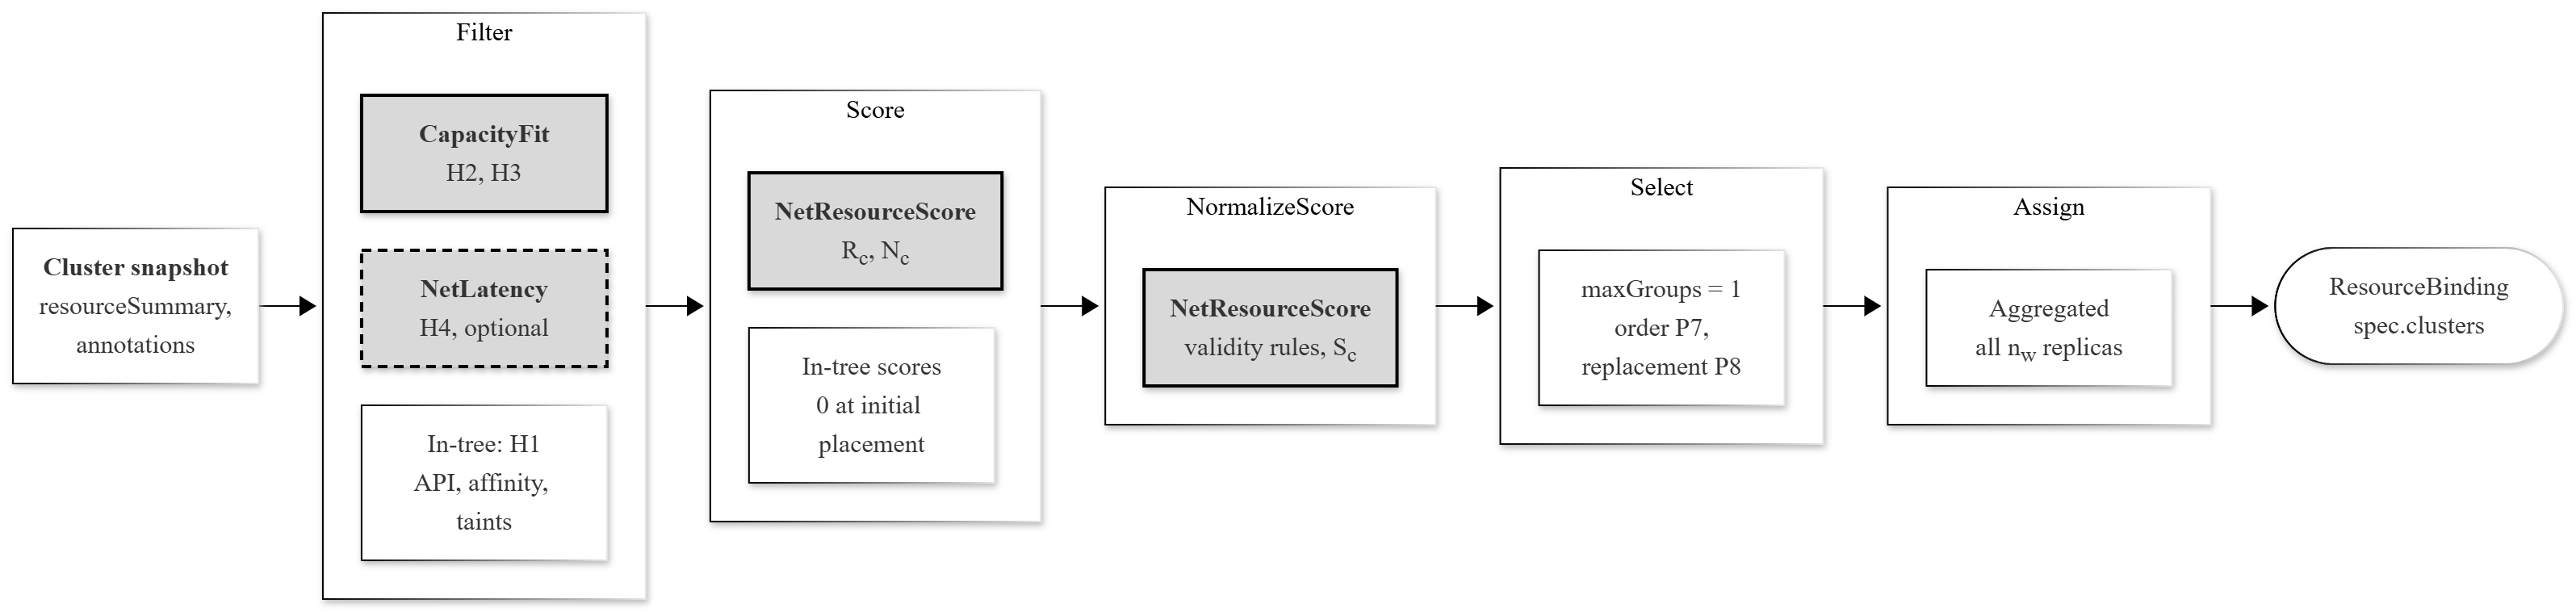
\includegraphics[width=\textwidth]{figures/pipeline.png}}% exported from figures/mermaid/pipeline.mmd
  {\resizebox{\textwidth}{!}{% Fig. 1 -- Karmada scheduling pipeline with the proposed plugins (shaded).
\begin{tikzpicture}[
  font=\footnotesize, >={Stealth[length=2mm]},
  stage/.style={draw, rounded corners=2pt, align=center, minimum width=2.2cm, minimum height=0.9cm, fill=white},
  prop/.style={draw, rounded corners=2pt, align=center, minimum width=2.2cm, minimum height=0.7cm, fill=gray!25, thick},
  exist/.style={draw, rounded corners=2pt, align=center, minimum width=2.2cm, minimum height=0.7cm, fill=white},
  lbl/.style={font=\scriptsize\itshape, align=center}
]
\node[stage] (snap) at (0,0) {Cluster\\snapshot};
\node[stage] (filt) at (3.0,0) {Filter};
\node[stage] (score) at (6.0,0) {Score};
\node[stage] (norm) at (9.0,0) {NormalizeScore};
\node[stage] (sel) at (12.0,0) {Select};
\node[stage] (asg) at (15.0,0) {Assign};

\foreach \a/\b in {snap/filt, filt/score, score/norm, norm/sel, sel/asg} \draw[->] (\a) -- (\b);
\draw[->] (asg.east) -- ++(0.7,0) node[right, lbl] {spec.\\clusters};

% plugins below each stage
\node[exist, below=0.5cm of filt] (f1) {in-tree: H1\\ \scriptsize affinity, taints, API};
\node[prop, below=0.25cm of f1] (f2) {CapacityFit\\ \scriptsize H2, H3};
\node[prop, dashed, below=0.25cm of f2] (f3) {NetLatency\\ \scriptsize H4 (optional)};
\node[exist, below=0.5cm of score] (s1) {in-tree scores\\ \scriptsize 0 at initial placement};
\node[prop, below=0.25cm of s1] (s2) {NetResourceScore\\ \scriptsize $R_c$, $N_c$};
\node[prop, below=0.5cm of norm] (n1) {NetResourceScore\\ \scriptsize validity rules, $S_c$};
\node[exist, below=0.5cm of sel] (sl1) {\code{maxGroups}=1\\ \scriptsize order P7,\\ \scriptsize replacement P8};
\node[exist, below=0.5cm of asg] (a1) {Aggregated\\ \scriptsize all $n_w$ replicas};
\node[exist, below=0.5cm of snap] (sn1) {resourceSummary,\\ \scriptsize annotations};

\foreach \s/\p in {snap/sn1, filt/f1, score/s1, norm/n1, sel/sl1, asg/a1} \draw[densely dotted] (\s.south) -- (\p.north);
\end{tikzpicture}
}}% TikZ fallback
\caption{Karmada scheduling stages and the position of the proposed plugins (shaded)}\label{fig:pipeline}
\end{figure}

\subsection{Algorithm}\label{sec:alg-algorithm}

\Cref{alg:netresource} gives the procedures of the three plugins. Score computes the resource term for each cluster separately, because Karmada calls it once per cluster. The validity rules of \cref{eq:score} depend on the whole candidate set, which in Karmada is visible only in the normalisation step (P1); the final score is therefore computed there. Every procedure returns a result for malformed input instead of an error.

\begin{algorithm}[t]
\caption{Filter, score and normalisation procedures of the proposed plugins}\label{alg:netresource}
\small\setstretch{1.0}
\begin{algorithmic}[1]
\Require binding with $n_w$, $d_w$; parameters $\alpha$, $\ell_{\mathrm{ref}}$, $\tau$, $q_{\min}$, vantage $v$, optional $\ell_{\max}$
\Procedure{CapacityFit}{$w, c$} \Comment{filter; H2, H3}
  \If{resource summary of $c$ is absent} \Return \textsc{Unschedulable} \EndIf
  \State $m \gets \min_{e \in E} e.\textsc{MaxAvailableReplicas}(c, w)$ \Comment{Karmada estimators}
  \If{$m < n_w$} \Return \textsc{Unschedulable} \EndIf
  \State \Return \textsc{Success}
\EndProcedure
\Procedure{NetLatency}{$w, c$} \Comment{optional filter; H4, fail-closed}
  \If{$\ell_{\max}$ not configured} \Return \textsc{Success} \EndIf
  \If{$\neg\,\textsc{Valid}(c, \mathrm{now})$ \textbf{or} $\ell_c > \ell_{\max}$} \Return \textsc{Unschedulable} \EndIf
  \State \Return \textsc{Success}
\EndProcedure
\Procedure{Score}{$w, c$} \Comment{called once per feasible cluster}
  \State $R \gets \operatorname{clip}\big(\min_{k} (A_c^k - U_c^k - P_c^k - n_w d_w^k)/A_c^k, 0, 1\big)$ \Comment{\cref{eq:resource}}
  \State \Return $\operatorname{round}(100 R)$ \Comment{provisional value}
\EndProcedure
\Function{Valid}{$c, t$}
  \State parse $\ell_c, t_c, q_c, v_c$ from the annotations of $c$; \textbf{if} parsing fails \Return \textbf{false}
  \State \Return $v_c = v \wedge q_c \geq q_{\min} \wedge t - t_c \leq \tau$ \Comment{\cref{eq:valid}}
\EndFunction
\Procedure{NormalizeScore}{list $L$ of (cluster, score)} \Comment{sees all candidates}
  \State $\Vset \gets \{ c \in L : \textsc{Valid}(c, \mathrm{now}) \}$
  \For{each $c \in L$}
    \State recompute $R_c$ from the snapshot \Comment{avoids rounding twice}
    \If{$\Vset = \emptyset$} $S_c \gets \operatorname{round}(100 R_c)$ \Comment{resource-only fallback; counted in a metric}
    \Else
      \State $N_c \gets \operatorname{clip}(1 - \ell_c/\ell_{\mathrm{ref}}, 0, 1)$ \textbf{if} $c \in \Vset$ \textbf{else} $0$ \Comment{missing is never favourable}
      \State $S_c \gets \operatorname{round}\big(100[\alpha R_c + (1-\alpha) N_c]\big)$
    \EndIf
  \EndFor
  \State \Return \textsc{Success}
\EndProcedure
\end{algorithmic}
\end{algorithm}

\subsection{Integration and configuration}\label{sec:alg-config}

The plugins are registered in a custom build of the Karmada scheduler through the out-of-tree registration function, and the parameters are passed as command-line options of that binary (P2) \cite{karmada_docs_custom_scheduler}. Because the score plugins are summed without weights (P3), the weighting of resource and network suitability is computed inside NetResourceScore and not by combining two plugins. The in-tree plugins remain enabled. At initial placement their scores are zero (P5), so the total score equals $S_c(w)$, and on a later rescheduling the existing locality preference of Karmada continues to apply unchanged.

Several scheduler instances can run side by side, each with its own scheduler name and leader-election lock \cite{karmada_docs_custom_scheduler}. This allows the same Karmada installation to offer the default behaviour, a resource-only configuration ($\alpha = 1$) and resource- and network-aware configurations ($0 < \alpha < 1$). A workload selects a configuration through the scheduler name in its PropagationPolicy, and removing the name returns it to the default scheduler. The same mechanism provides the comparison setting of the validation plan in \cref{sec:validation}.

Two configuration details affect correctness. First, when resource models are enabled with the default grades, clusters composed of small nodes are underestimated (\cref{sec:method-capacity}); such installations should define finer models or enable the accurate estimator. Second, until the pods of a newly placed workload appear in the member cluster, its demand is absent from the resource summary. Karmada can account for such in-flight placements through a feature gate that is alpha and disabled by default in v1.19.1. Without it, several placements made within one status interval may select the same cluster. This affects the default scheduler in the same way.
